\documentclass[main.tex]{subfiles}

\begin{document}

\begin{table}[h!]
	\centering
	
	\begin{tabular}{l|l|l|l}
		\toprule
		Model name & Top-1 acc. & Training time (sec) & Inference speed (img/sec) \\
		\midrule
		Logistic Regression${}^\dagger$ & 0.92 & 0.28 & 257231 \\
		\midrule
		SVM (Linear) & 0.93 & 0.02 & 72707 \\
		SVM (Gaussian) & 0.95 & 0.04 & 20958 \\
		SVM (Sigmoid) & 0.85 & 0.11 & 11992 \\
		SVM (Polynomial deg2) & 0.95 & 0.03 & 49184 \\
		SVM (Polynomial deg3) & \textbf{0.97} & 0.03 & 54403 \\
		\midrule
		FDA & 0.91 & 0.01 & 767676 \\
		\midrule
		MLP${}^\dagger$ & 0.93 & 0.49 & 603443 \\
		CNN${}^\dagger$ & \textbf{0.97} & 2.31 & 249295 \\
		\bottomrule
	\end{tabular}

	\vspace{0.2cm}
	\caption{Comparison between the algorithms. Training time and inference speed measured on an Intel i9-10940X CPU. MLP and CNN were implemented using PyTorch, and the rest were implemented using scikit-learn. $\dagger$Allowed to use multi-threading in inference and training.}
	\label{modelcomp}
\end{table}

In following sub-sections, we will show the comparison between algorithms in two perspective: efficiency, and translation invariance.

\subsection{Efficiency}

Efficiency does not simply mean speed.
Basically, it can be said that a model with a high accuracy guaranteed
and an acceptable speed is efficient.
From this point, the most efficient models are the Support Vector Machine with Polynomial kernel of degree 3 and the Convolutional Neural Network.
In Table \ref*{modelcomp}, Support Vector Machine with Polynomial kernel with degree 3 and Convolutional Neural Network are the most accurate with 97\% accuracy.
However, there is a big difference between the two algorithms in terms of time.
The training speed is about 80 times faster in Support Vector Machine with Polynomial kernel with degree 3 than in Convolutional Neural Network.
The inference speed is about five times faster for Convolutional Neural Network.
The difference in the training time is due to the fact that Convolutional Neural Network requires a lot more calculations compared to Support Vector Machine.
On the other hand, because batch operations that process multiple samples at once are supported in Convolutional Neural Network, there is a difference in the inference speed.
Therefore, Convolutional Neural Network and Support Vector Machine with Polynomial kernel with degree 3 are both efficient, depending on which one we focus on.

\subsection{Translation Invariance}
\begin{figure}[H]
	\centering
	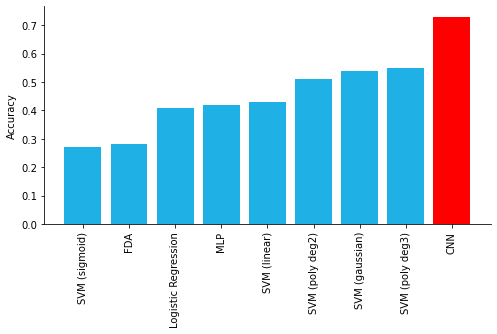
\includegraphics[scale=0.5]{img/result/translate_acc.png}
		
	\caption{Accuracy of each model on translated validation dataset.}
	\label{translatefig}
\end{figure}

Translation invariance is one of the important things for computer vision tasks.
Computer Vision problems are finding important information among given images.
However, the information does not always appear in the same location in the image.
It may be in the middle of the image or may be biased in one direction.
Hence, being strong against translation means that the generalization performance of the model is excellent.

Fig. \ref*{translatefig} demonstrates the generalization performance of each model for translation.
Convolutional Neural Network has the most overwhelming performance compared to other models.
On the other hand, Support Vector Machine with Polynomial kernel of degree 3, which showed similar accuracy to Convolutional Neural Network in the original validation dataset,
significantly decreased performance in the translated validation set.
Since not all models have experienced data that are not centered in the training process,
these results imply that Convolutional Neural Network has better generalization power for computer vision.

\end{document}
